\section{Analisi dei dati}\label{sec:analisi}
\normalsize
In questa sezione saranno analizzati i dati di SkillCraftI \cite{SkillCraft} per cercare di capire la struttura dei dati e correggere eventuali problemi che il dataset potrebbe avere. Durante questa analisi saranno usate le librerie Python Matplotlib e Seaborn per graficare i dati e renderli più interpretabili.   
\subsection{Bilanciamento del dataset}\label{ssec:bilanciamento}
\normalsize
\par
Le leghe di Starcraft sono per loro natura sbilanciate.
Dal sito Liquipedia \cite{liquipedia}, un'enciclopedia online a tema videogiochi, si può leggere come queste siano strutturate e gli obbiettivi che si sono posti gli sviluppatori quando le hanno create. \\*\\*
La distribuzione a cui puntavano gli sviluppatori è come segue: 
\begin{itemize}
	\item Grand Master 1000 giocatori
	\item Master 2\%
	\item Diamante 18\%
	\item Platino 20\%
	\item Oro 20\%
	\item Argento 20\% 
	\item Bronzo 20\%
\end{itemize}

Nella realtà le cifre sono destinate ad essere leggermente diverse, ma la proporzione è a grandi line corretta. In più, oltre alle leghe del gioco, nel data set possiamo trovare anche i giocatori professionisti. Questa ulteriore divisione è stata aggiunta perché anche se i Grand master possono essere considerati un élite tra i giocatori, il divario tra le loro capacità e quelle dei professionisti è considerevole.\\*
Le proporzioni del database Skillcraft invece sono indicate nel grafico a seguire \ref{fig:dist}. \\*\\*
\begin{figure}[h]
	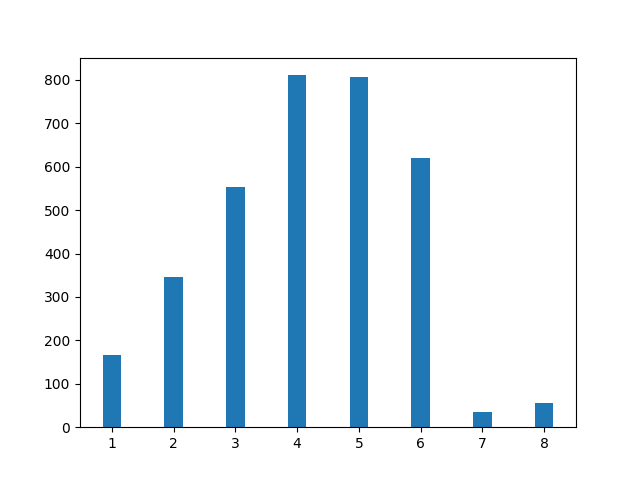
\includegraphics[scale=0.9]{../figures/sbilanciamento.PNG}
	\caption{Distribuzione sample nelle leghe}
	\label{fig:dist}
\end{figure}
\par
Come previsto il dataset è sbilanciato, e ciò comporta una maggiore attenzione alle modalità di raggruppamento dei campioni durante l'addestramento dei modelli e nello splitting. Oltre a questo, l'unica altra anomalia che è possibile individuare è che le ultime tre leghe sono più numerose di quello che dovrebbero essere. Tale anomalia non è rispecchiata nella realtà ed è dovuto al modo in cui sono stati campionati i dati, ma ai fini della classificazione non dovrebbe creare grossi problemi.
\clearpage
\subsection{Elementi nulli}\label{ssec:nulli}
\normalsize
\par
Per la buona riuscita dell’addestramento è necessario rimuovere tutti gli elementi nulli, e il nostro dataset ne contiene alcuni. Ora cercheremo di capire quanti sono e come sono distribuiti per trovare una soluzione al problema.\\*\\*
Il grafico sotto rappresenta il numero totale di elementi nulli per ogni lega, divisi per la feature a cui appartengono.\\*
\begin{figure}[h]
	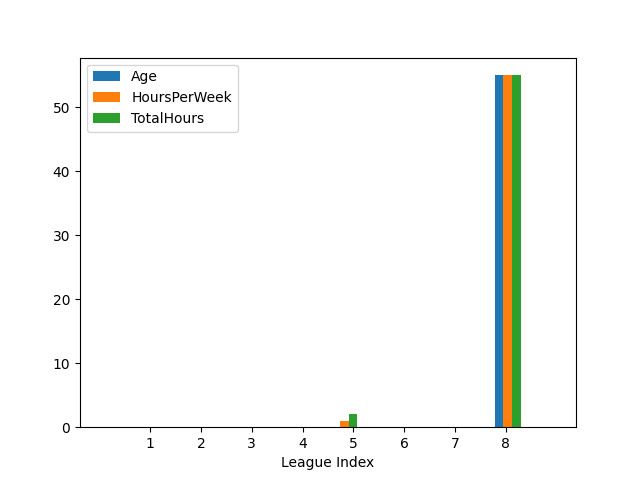
\includegraphics[scale=0.9]{../figures/Nan_distribuzione.PNG}
	\caption{Distribuzione elementi nulli}
\end{figure}
\par
Dal grafico si può vedere che gli elementi nulli sono concentrati in 3 features che rappresentano: Età, ore di gioco settimanali e ore di gioco totali. Inoltre, la maggior parte è inserito nella lega 8, ovvero i professionisti. \\*\\*
Esistono diverse soluzioni per gestire gli elementi nulli di un dataset, ad esempio si possono eliminare le righe che ne contengono uno, ma nel nostro caso, controllando i dati dei professionisti si può notare che le tre colonne identificate prima sono tutte nulle in questa lega, di conseguenza eliminare le righe con elementi nulli vorrebbe dire perdere completamente i dati sui professionisti.\\*\\*
Un’altra alternativa è quella di riempire i dati nulli con un valore che potrebbe stimarli, come la media degli altri valori di quella feature in quella lega, ma come visto prima non ci sono altri valori su cui costruire la stima e di conseguenza questa strada è impraticabile.\\*\\*
L’unica alternativa rimasta è eliminare le colonne con i valori nulli, e per misurare l’effetto che questa decisione avrà sulla classificazione possiamo sfruttare una mappa di correlazione\\*\\*
La mappa di correlazione rappresenta le relazioni tra gli elementi su cui è costruita, da essa è possibile capire quanto due feature sono legate tra di loro e con la classe che vogliamo predire.\\*
\begin{figure}[htp]
	\makebox[\textwidth][c]{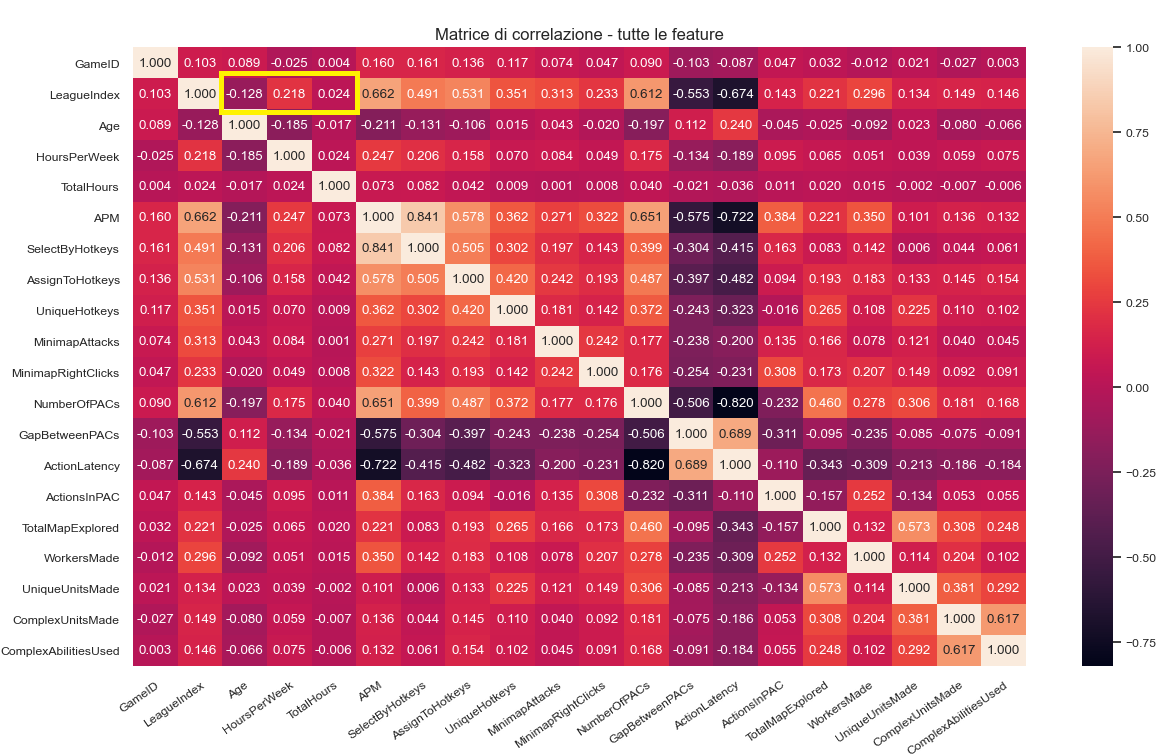
\includegraphics[scale=0.6]{../figures/correlation totale corretta.PNG}}
	\caption{Mappa di correlazione}
\end{figure}
\par
I valori evidenziati in giallo sono gli indici di correlazione delle feature che contengono i valori nulli, fortunatamente sono tendenzialmente bassi, quindi togliendoli non andremo ad influire sulla classificazione, ma potremmo addirittura migliorare le prestazioni di certi algoritmi di classificazione.
\clearpage

\subsection{Relazioni tra le feature}\label{ssec:relazioni}
\normalsize
\par
A questo punto bisogna controllare come sono fatte le feature, che relazioni hanno tra di loro e in particolare con il target da classificare.\\*\\*
Per farlo useremo principalmente due grafici: il pairplot e la matrice di correlazione vista prima. Il primo ci serve a definire il tipo di relazione, mentre la seconda da un'indicazione più quantitativa della relazione.\\*\\*
Il pairplot può essere usato per guardare le relazioni tra tutte le feature, ma nel nostro caso è sconveniente vista l’elevata quantità di esse, perché i grafici verrebbero troppo piccoli e disordinati per essere comprensibili. Quindi ho deciso di fare un pairplot con solo le relazioni delle feature con il target, ovvero l’indice della lega.
\begin{figure}[htp]
	\makebox[\textwidth][c]{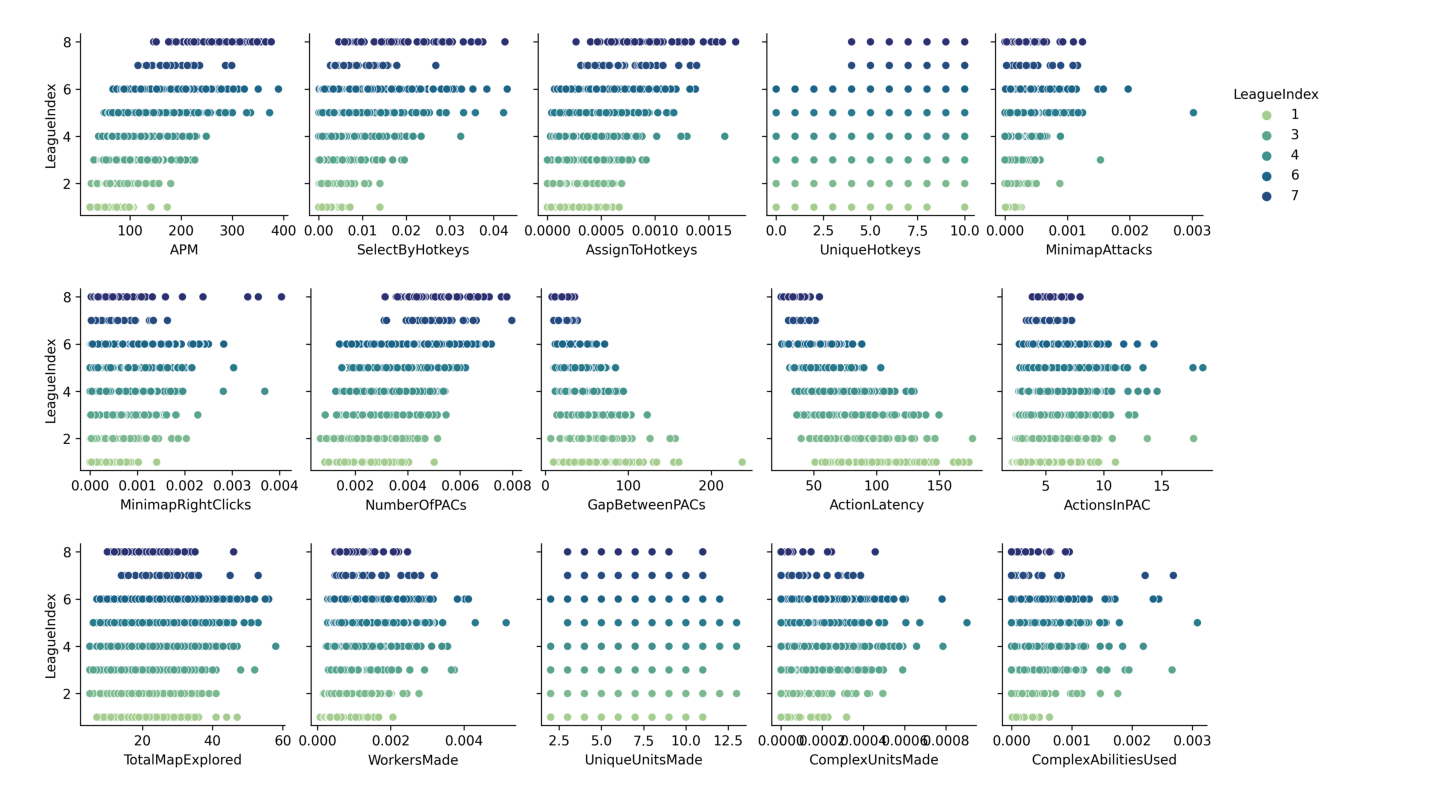
\includegraphics[scale=0.5]{../figures/pairplot_features_target.PNG}}
	\caption{Pairplot delle feature con il target}
\end{figure}
\par
Le cose che possiamo notare dai grafici sono due:
\begin{itemize}
	\item La prima è che guardando il pairplot possiamo notare che alcune features hanno dei pattern nella loro relazione con il target, in particolare l’APM e l’ActionLatency, che sono anche le due feature con la correlazione maggiore, sembrano seguire un andamento vagamente lineare.
	\item La seconda riguarda la mappa di correlazione, dove possiamo notare che alcune features hanno una correlazione forte tra di loro, che è un indice di collinearità e multicollinearità. Questi fenomeni sono abbastanza pericolosi perché rendono i modelli suscettibili al rumore delle feature.
\end{itemize}
Analizzando questo il problema della multicollinearità a fondo però è possibile rendersi conto che queste feature, sebbene collegate, non sono l’una la diretta conseguenza dell’altra. Prendendo ad esempio le APM e il numero di selezioni fatte con tasti personalizzati, l’usare dei tasti personalizzati, se fatto male può portare anche al calo degli APM dovuto al tempo necessario per correggere gli errori, quindi l'abilità di fare queste operazioni correttamente è un buon indice della qualità di un giocatore.\\*\\*
Visto che anche gli altri casi sono simili a questo, ovvero anche se c'è correlazione il modo in cui sono correlati può essere significativo alla classificazione, ho deciso di lasciare inizialmente tutte le feature. Se poi durante l'analisi dei risultati avessi trovato la conferma che questo peggiora i risultati, allora sarei tornato indietro a avrei fatto una maggiore feature selection, ma non è stato così.\\*\\*

